\section{VIA Architecture}
\label{sec:via:arch}

\begin{figure}[t!]
\centering
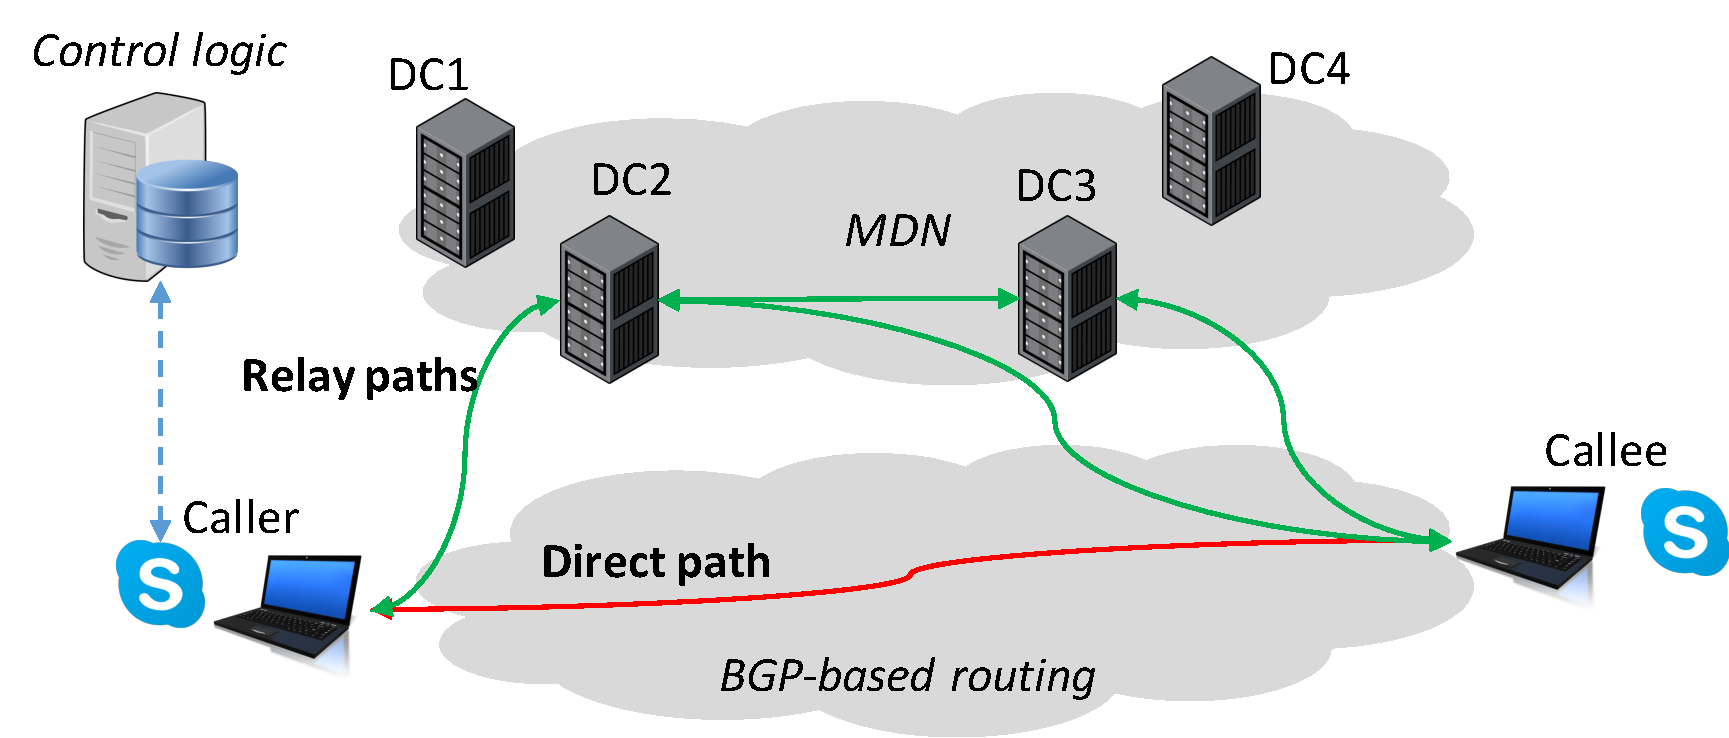
\includegraphics[width=0.7\textwidth]{figures/Via-MdnOverview.pdf}
\caption{\hybrid architecture with relay nodes at globally distributed data centers. A call can either take ``\direct path'' (red) or a ``relay path'' (green).}
%\ga{Callee to controller line.}
\label{fig:mdn-overview}
\end{figure}

Figure~\ref{fig:mdn-overview} presents the \hybrid architecture that consists of relay nodes placed at globally distributed datacenters, such as those run by Amazon, Google, and Microsoft. 
Indeed, {\hybrid}'s architecture bears similarities to those used by Google Hangouts and Skype~\cite{VideoTelephony-IMC12}, but with a key difference --- today, the relays are typically used to provide connectivity between any two clients, while \hybrid is engineered to {\em explicitly} optimize network performance and call quality.
%Indeed, this architecture bears similarities to that used by Google Hangouts and Skype~\cite{VideoTelephony-IMC12}, albeit primarily for connectivity (i.e., firewall and NAT traversal) rather than performance optimization (which is our focus here).

Each call can take either the ``{\em \direct} path'' (red arrow) or a ``{\em relayed} path'' (green arrows) that routes the traffic through one or more relay nodes in the DCs. Relayed paths could include a single relay to "{\em bounce} off" traffic or a pair of relays to enable traffic to "{\em transit} through" the private backbone of the managed overlay network. 


%%%%In our study, we use $74$ relay nodes, all located in a single AS\camera{ (so all inter-relay paths are across a private WAN)} and operated by \skype but spread across large datacenters and edge clusters in $30$ countries across $5$ continents. 
In our study, we use all the relay nodes operated by \skype. They are all located in a single AS (so all inter-relay paths are within a private WAN) but spread across many tens of datacenters and edge clusters worldwide. 
We assume the caller (or callee) can reach these relays %either through a shared anycast address, by letting the underlying network routing pick the "closest" relay, or 
by explicitly addressing the particular relay(s). %\camera{In this work, we assume the latter.} %\vnp{I'm confused by the previous sentence --- isn't Via all about explicitly selecting the relays?}
%In any case, since the relays are all in the same AS, the inter-domain path is determined by BGP. 
The network path between a relay and a client is determined by BGP. 
%While we could have considered approaches such as having a regionally-advertised IP block for each relay, to enable greater control over the {\em path} to each relay, we explicitly avoided these for ease of deployment.\vnp{The previous sentence can be deleted if we need to save space}

% Relaying audio calls through a \managed is feasible and is likely to provide better performance than BGP on international and interdomain calls, since large entities such as Amazon and Microsoft own geo-distributed DCs and edge clusters with high-quality backbone connectivity between them.

% The architecture in Figure~\ref{fig:mdn-overview} is generic and bear many similarities to the one that is being operated by Google Hangouts and Skype~\cite{imc-skype-study}. Based on data from \skype, we use $74$ relay nodes that are located across large datacenters and edge clusters, spread over \fillme countries. 

% Relayed calls typically traverse two relay nodes. The packets from the caller enter the \managed via a (nearby) {\em ingress} relay node, which in turn routes the packet via the private backbone to an egress relay that is close to the callee. Transparent to both the end-points, the call might internally traverse other relay nodes. Depending on the network characteristics, calls might also be {\em bounced off} just a single relay. The route between the end-points and the relays is either via anycast (wherein a common addressed is advertised from all the peering locations) or by explicitly picking from a set of regionally-advertised IP addresses, each corresponding to a specific relay. We explicitly avoided approaches that require control of the path to the relay for ease of deployability.

When establishing a call, after the caller signals its callee, both the caller and callee contact a {\em controller} (Figure~\ref{fig:mdn-overview}) to determine whether they should use the direct path or a relayed path, and, in case of the latter, which relay(s) they should use. The controller makes this decision based on the performance measurements from historical calls and policy constraints (such as those based on relay budget or current load), to be described in Section~\ref{sec:via:design}. To aid in this process, \skype clients periodically push the network metrics derived from their calls, to the controller. 
%As Section~\ref{sec:motivation} motivated, the controller dynamically updates its decisions using the latest measurements. 

The controller does not need to directly monitor the relay nodes because their performance (including degradation and failure) would be reflected in the end-to-end measurements made by clients who use the relays. %\footnote{In addition to the end-to-end measurements, we also rely on network performance measurements between the relay nodes, as explained in \Section~\ref{subsec:potential-overall}}.}
To avoid overloading the controller, each client could cache the relaying decisions and refresh periodically though we do not consider this here. (We 
 discuss implementation issues in Section~\ref{sec:via:discussion}). %in this paper.
%\ga{Cache results to avoid going to the controller?}
% , and returns as output the selection of relay or direct path for each call. 
%A naive control logic would be to have all calls relayed through the same relay nodes. However, since many BGP paths only have quality issues for a small fraction of time (see Figure~\ref{fig:temporal-structure}), it would be desirable to have a dynamic decision algorithm that select paths depending on when and between which nodes a call is being placed.
